
%	======= 1) NOW WHAT? =======

\begin{frame}
	\frametitle{Muy bien pero...¿Cómo sigo?}
	
	\begin{center}
		
\includegraphics[scale=0.40]{img/nowwhat.jpg}
	\end{center}

\end{frame}

%	======= 2) REQUISITOS =======

\begin{frame}
	\frametitle{¿Qué necesito?}
	
	Como has podido ver desarrollar un videojuego no es tarea fácil, requiere de un proceso de constante aprendizaje, investigación, dedicación y mucha ayuda.
		
	\begin{block}{Recomendaciones}
		\begin{itemize}
			\item Motivación: Hay que dedicarle mucho tiempo.
			\item Curiosidad: Interés por aprender cosas nuevas y mejorar lo que ya sabes.
			\item Saber Inglés: Gran cantidad de los recursos de calidad están en inglés.
			\item Contactos: Trabajo artístico, publicitario, sonido, beta testers...
			\item Comunidad: Lugar de referencia para consultar, compartir, etc.
		\end{itemize}
	\end{block}

\end{frame}

%	======= 3) LENGUAJES =======

\begin{frame}
	\frametitle{Lenguajes Alto Nivel}
	
	Según los conocimientos que tengas, así como los propósitos y metas del juego a desarrollar es importante elegir bien el lenguaje de programación.
		
	\begin{block}{Recomendaciones}
		\begin{itemize}
			\item C/C++/C\#
			\item Python
			\item Java
			\item Lua
			\item Lisp
			\item Ruby
		\end{itemize}
	\end{block}

\end{frame}

%	======= 4) LIBRERÍAS 2D =======

\begin{frame}
	\frametitle{Librerías 2D}
		
	La mejor forma de adentrarse en el desarrollo de videojuegos.
	\newline
	\begin{block}{Algunos ejemplos destacados}
		\begin{itemize}
			\item Gosu
			\item SDL
			\item Allegro
			\item Pygame
			\item ClanLib
		\end{itemize}
	\end{block}

\end{frame}

%	======= 5) LIBRERÍAS 3D =======

\begin{frame}
	\frametitle{Librerías 3D}
	\begin{columns}[c]
		\column{150pt}
			El salto de calidad...
		\column{150pt}
			\begin{center}
				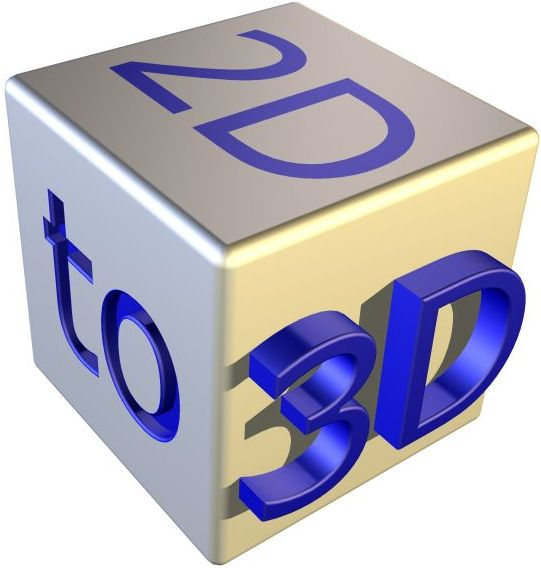
\includegraphics[scale=0.05]{img/2dto3d.jpg}
			\end{center}
	\end{columns}
	\begin{block}{Algunos ejemplos destacados}
		\begin{itemize}
			\item Ogre
			\item IrrLicht
			\item Crystal Space
			\item Panda
		\end{itemize}
	\end{block}

	\begin{center}
		
\includegraphics[scale=0.45]{img/logos.png}
	\end{center}

\end{frame}

%	======= 6) LIBRERÍAS AUXILIARES =======

\begin{frame}
	\frametitle{Otras Librerías y Herramientas}
		
	En muchas ocasiones es necesario apoyarse en otras librerías externas o herramientas que desarrollarán funciones auxiliares.
	\newline
	\begin{block}{Algunos ejemplos destacados}
		\begin{itemize}
			\item Física: ODE, BULLET.
			\item Gestión de Entrada: OIS.
			\item Diseño Artístico: Gimp, Blender.
		\end{itemize}
	\end{block}

\end{frame}

%	======= 7) RECURSOS BIBLIOGRÁFICOS =======

\begin{frame}
	\frametitle{La biblioteca}
	
	\begin{center}
		
\includegraphics[scale=0.50]{img/biblio.jpg}
	\end{center}

\end{frame}

%	======= 8) TRABAJO EN EQUIPO =======

\begin{frame}
	\frametitle{Trabajo en Equipo}
	
	\begin{center}
		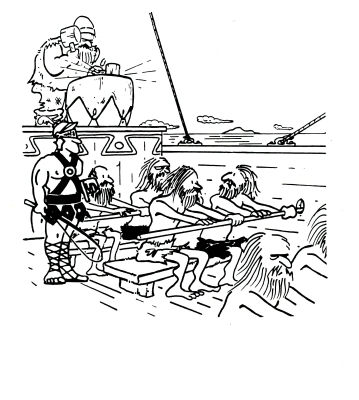
\includegraphics[scale=0.70]{img/equipo.jpg}
	\end{center}

\end{frame}

%	======= 9) ADVUCA, TU AMIGO FIEL =======

\begin{frame}
	\frametitle{ADVUCA}
		
	Desde la ADVUCA nos comprometemos a ofrecer ayuda para fomentar desarrollo de proyectos e incentivar el aprendizaje a través de los videojuegos.

	\begin{block}{Algunos ejemplos destacados}
		\begin{itemize}
			\item Formación de grupos de trabajo(juegos, manuales, etc).
			\item Difusión.
			\item Consultas.
		\end{itemize}
	\end{block}

	\begin{center}
		
\includegraphics[scale=0.50]{img/micro.png}
	\end{center}

\end{frame}

%	======= 10) MUNDO LABORAL =======

\begin{frame}
	\frametitle{El Exterior...}
		
	Después de la UCA, empieza lo bueno...
	\newline
	\begin{columns}[c]
		\column{150pt}
			\begin{block}{Algunas posibilidades}
				\begin{itemize}
					\item Masters.
					\item Desarrolladoras de Videojuegos.
					\item Centros Multimedia.
				\end{itemize}
			\end{block}
		\column{150pt}
			\begin{center}
				
\includegraphics[scale=0.15]{img/exterior.jpg}
			\end{center}
	\end{columns}
\end{frame}


